\documentclass{ctexart}
\usepackage[utf8]{inputenc}
\usepackage{amsmath}
\usepackage{graphicx}

\title{数值分析 - 第二次上机作业 - 实验报告}
\author{樊睿\\强基数学 2001 班}
\date{October 10,2022}

\begin{document}

\maketitle

\begin{abstract}
本文详细介绍了 Newton 插值、Hermite 插值、Chebyshev 插值法的实现,并用它们解决了一些实际问题。
\end{abstract}

\section{多项式函数类}
本章将用到多项式。为了在计算机中合理地存储任意次的多项式,我们有必要先实现多项式函数类。

多项式首先是函数,所以它要继承第一章的仿函数类,并继承它的两个虚函数求函数值和求导数值。$n$ 次多项式要存储 $0$ 到 $n$ 次项系数,可用一个 \verb|vector| 存储。

因此,多项式函数类要从仿函数类和 \verb|vector| 类同时继承。无需定义更多成员变量。定义成员函数 \verb|time| 求多项式的次数。

本章将用到多项式的加法、数乘和乘法运算,因此要对多项式类重载这三个运算。还需要对多项式求导(返回导函数而非一个导数值),因此也重载了函数 \verb|d|。

多项式的输出使用 \verb|a0+a1*x+a2*x**2+...+an*x**n| 的格式,方便后期在 python 中作图。

代码如下。

注,这段代码有一些问题没有解决:暂时不能用一个 \verb|vector| 去初始化多项式。即 \verb|Polynomial<double> p({1})| 是无法通过编译的。

\begin{verbatim}
template <class type> 
class Polynomial : public vector <type>, public Function <type> {
public :
    Polynomial (const int & n = -1, const type & x0 = 0, const type & x1 = 0) {
        this -> resize(n+1);
        if (n >= 0) this -> at(0) = x0;
        if (n >= 1) this -> at(1) = x1;
    }
    int time() const {
        return this -> size() - 1;
    }
    Polynomial <type> operator + (const Polynomial <type>& b) const {
        int n = max(time(), b.time()), m = min(time(), b.time());
        Polynomial <type> c(n);
        for (int i = 0; i <= m; ++ i) c[i] = this -> at(i) + b[i];
        if (n == time())
            for (int i = m+1; i <= n; ++ i) c[i] = this -> at(i);
        else
            for (int i = m+1; i <= n; ++ i) c[i] = b[i];
        return c;
    }
    Polynomial <type> operator += (const Polynomial <type>& b) {
        return *this = *this + b;
    }
    Polynomial <type> operator * (const type& b) const {
        int n = time();
        Polynomial <type> c(n);
        for (int i = 0; i <= n; ++ i) c[i] = this -> at(i) * b;
        return c;
    }
    Polynomial <type> operator *= (const type & b) {
        return *this = *this * b;
    }
    Polynomial <type> operator * (const Polynomial <type>& b) const {
        int n = time(), m = b.time();
        Polynomial <type> c(n+m);
        for (int i = 0; i <= n; ++ i)
            for (int j = 0; j <= m; ++ j)
                c[i+j] += this -> at(i) * b[j];
        return c;
    }
    Polynomial <type> operator *= (const Polynomial <type>& b) {
        return *this = *this * b;
    }
    virtual type operator ()(const type & x) const {
        int n = time();
        type res = 0;
        for (int i = n; i >= 0; -- i)
            res = res * x + this -> at(i);
        return res;
    }
    Polynomial <type> d() {
        int n = time();
        Polynomial <type> c(n-1);
        for (int i = n; i > 0; -- i)
            c[i-1] = this -> at(i) * i;
        return c;
    }
    virtual type d(const type & x) const {
        int n = time();
        type res = 0;
        for (int i = n; i > 0; -- i)
            res = res * x + this -> at(i) * i;
        return res;
    }
};

template <class type>
Polynomial <type> operator * (const type & x, const Polynomial <type> & p) {
    return p * x;
}

template <class type>
ostream & operator << (ostream &out, const Polynomial <type> &p) {
    int n = p.time();
    if (n == -1) {cout << 0; return out;}
    for (int i = 0; i <= n; ++ i) {
        out << p[i];
        if (i == 1) out << "*x";
        else if (i >= 2) out << "*x**" << i;
        if (i < n) {
            if (p[i+1] >= 0) out << " +";
            else cout << " ";
        }
    }
    return out;
}
\end{verbatim}

\section{Newton 插值}

\subsection{算法的实现}
输入插值点 $(x_0,y_0),(x_1,y_1),\dots,(x_n,y_n)$,满足对任意 $i\neq j$ 均有 $x_i\neq x_j$。输出 $n$ 次插值多项式 $p_n(x)$,满足对任意 $0\leq i\leq n$,均有 $p_n(x_i)=y_i$。

根据课本 Def 2.18,需要 $O(n^2)$ 的时空来计算差商表;然后根据课本 Def 2.14 用 $O(n^2)$ 的时间计算插值多项式的表达式。但若不需要计算表达式,则只需 $O(n)$ 的时间计算插值多项式的一个点值。

源码如下:

\begin{verbatim}
template <class type>
class Newton_Interpolation {
private:
    vector <type> x, y;
    vector <vector <type>> f;
public:
    Newton_Interpolation(const vector <type>& x, const vector <type>& y) : x(x), y(y) {
        int n = x.size() - 1;
        f.resize(n+1);
        for (int i = 0; i <= n; ++ i) f[i].resize(n+1);
        for (int i = 0; i <= n; ++ i) f[i][i] = y[i];
        for (int j = 1; j <= n; ++ j) {
            for (int i = 0; i <= n-j; ++ i)
                f[i][i+j] = (f[i+1][i+j] - f[i][i+j-1]) / (x[i+j] - x[i]);
        }
    }
    type GetValue(const type& _x) const {
        int n = x.size() - 1;
        type res = 0, pi = 1;
        for (int i = 0; i <= n; ++ i) {
            res += f[0][i] * pi;
            pi *= _x - x[i];
        }
        return res;
    }
    Polynomial <type> GetPolynomial() const {
        int n = x.size() - 1;
        Polynomial <type> res(0, 0), pi(0, 1);
        for (int i = 0; i <= n; ++ i) {
            res += f[0][i] * pi;
            pi *= Polynomial <type>(1, -x[i], 1);
        }
        return res;
    }
};
\end{verbatim}

\subsection{在均匀网格上 Newton 插值}
输入函数、左右区间、插值点数,输出插值多项式。源码如下:

\begin{verbatim}
Newton_Interpolation <double> Grid_Interpolation (const Function <double> & f, const double & l, const double & u, const int & n) {
    vector <double> x(n+1), y(n+1);
    for (int i = 0; i <= n; ++ i) {
        double xi = l + (u - l) * i / n;
        double yi = f(xi);
        x[i] = xi, y[i] = yi;
    }
    return Newton_Interpolation<double>(x, y);
}
\end{verbatim}

\subsection{Chebyshev 插值}
输入函数、左右区间、插值点数,输出插值多项式。

根据 Thm 2.44 计算 Chebyshev 插值点 $x_0,x_1,\dots,x_n$。源码如下:

\begin{verbatim}
Newton_Interpolation <double> Chebyshev_Interpolation (const Function <double> & f, const double & l, const double & u, const int & n) {
    vector <double> x(n+1), y(n+1);
    for (int i = 0; i <= n; ++ i) {
        double xi = (u + l) / 2 + (u - l) / 2 * cos(PI*(2*i+1)/(2*(n+1)));
        double yi = f(xi);
        x[i] = xi, y[i] = yi;
    }
    return Newton_Interpolation<double>(x, y);
}
\end{verbatim}

\section{Hermite 插值}

输入插值点 $(x_0,y_0,y_0^{(1)},\dots,y_0^{(m_0)}),(x_1,y_1,y_1^{(1)},\dots,y_1^{(m_1)}),\dots,(x_n,y_n,y_n^{(1)},\dots,y_n^{(m_n)})$,输出插值多项式 $p_N$,满足对任意 $0\leq i\leq n,0\leq j\leq m_i$,均有 $p_N^{(j)}(x_i)=y_i^{(j)}$。

但若直接按课本中问题描述的形式输入插值点,在存储插值点和后续计算差商表时都会非常困难。因此在实际输入时,不输入二维的插值点及其导数值的列表,而是仍采用和 Newton 插值相同的输入格式,以一维数组的格式给出 $(x_0,y_0),(x_0,y_0^{(1)}),\dots$。例如若插值多项式要满足 $p(0)=0,p'(0)=1,p''(0)=2,p(1)=1,p(2)=3,p'(2)=5$,则输入的数据为 $x=\{0,0,0,1,2,2\},y=\{0,1,2,1,3,5\}$。

这样在计算差商表中 $f[x_i,\dots,x_j]$ 的值时,若 $x_i\neq x_j$,直接使用 Def 2.18 的公式计算即可;若 $x_i=x_j$,则根据 Cor 2.36 从 $y$ 中直接取相应高阶导数值并除以阶数的阶乘即可。这里可能需要辅助数组来存储每个 $x_i$ 在输入的 $x$ 数组的起始位置。

\begin{verbatim}
template <class type>
class Hermite_Interpolation {
private:
    vector <type> x, y;
    vector <vector <type>> f;
public:
    Hermite_Interpolation(const vector <type>& x, const vector <type>& y) : x(x), y(y) {
        int n = x.size() - 1;
        f.resize(n+1);
        for (int i = 0; i <= n; ++ i) f[i].resize(n+1);
        vector <int> m(n+1);
        for (int i = 0; i <= n; ++ i) {
            if (!i || x[i] != x[i-1]) m[i] = i;
            else m[i] = m[i-1];
        }
        for (int i = 0; i <= n; ++ i) f[i][i] = y[m[i]];
        vector <type> fac(n);
        fac[0] = 1;
        for (int i = 1; i <= n; ++ i) fac[i] = fac[i-1] * i;
        for (int j = 1; j <= n; ++ j)
            for (int i = 0; i <= n-j; ++ i) {
                if (x[i+j] == x[i]) f[i][i+j] = y[m[i]+j] / fac[j];
                else f[i][i+j] = (f[i+1][i+j] - f[i][i+j-1]) / (x[i+j] - x[i]);
            }
    }
    type GetValue(const type &_x) const {
        int n = x.size() - 1;
        type res = 0, pi = 1;
        for (int i = 0; i <= n; ++ i) {
            res += f[0][i] * pi;
            pi *= _x - x[i];
        }
        return res;
    }
    Polynomial <type> GetPolynomial() const {
        int n = x.size() - 1;
        Polynomial <type> res(0, 0), pi(0, 1);
        for (int i = 0; i <= n; ++ i) {
            res += f[0][i] * pi;
            pi *= Polynomial <type>(1, -x[i], 1);
        }
        return res;
    }
};
\end{verbatim}

\section{问题求解}

\subsection{第二题,Runge 现象}
首先定义函数 $f(x)=\dfrac 1{1+x^2}$。
\begin{verbatim}
class F1 : public Function <double> {
public:
    virtual double operator () (const double &x) const {
        return 1 / (x * x + 1);
    }
} f1;
\end{verbatim}

然后按题意进行求解。
\begin{verbatim}
    Newton_Interpolation<double> ip1_2 = Grid_Interpolation(f1, -5, 5, 2);
    Newton_Interpolation<double> ip1_4 = Grid_Interpolation(f1, -5, 5, 4);
    Newton_Interpolation<double> ip1_6 = Grid_Interpolation(f1, -5, 5, 6);
    Newton_Interpolation<double> ip1_8 = Grid_Interpolation(f1, -5, 5, 8);
    Polynomial<double> p1_2 = ip1_2.GetPolynomial();
    Polynomial<double> p1_4 = ip1_4.GetPolynomial();
    Polynomial<double> p1_6 = ip1_6.GetPolynomial();
    Polynomial<double> p1_8 = ip1_8.GetPolynomial();
    cout << p1_2 << endl;
    cout << p1_4 << endl;
    cout << p1_6 << endl;
    cout << p1_8 << endl;
\end{verbatim}

将输出的多项式值复制到 python 程序中,在 $[-5,5]$ 中均匀取 $1000$ 个点作图。

\begin{verbatim}
import matplotlib.pyplot as plt
import numpy as np

def f(x) :
    return 1 / (1 + x**2)
def p2(x) :
    return 1 - 0.0384615*x**2
def p4(x) :
    return 1 - 0.171088*x**2 + 0.00530504*x**4
def p6(x) :
    return 1 - 0.351364*x**2 + 0.0335319*x**4 - 0.000840633*x**6
def p8(x) :
    return 1 - 0.528121*x**2 + 0.0981875*x**4 - 0.00658016*x**6 + 0.000137445*x**8

x = np.linspace(-5, 5, 1000)
y = [f(t) for t in x]
plt.plot(x, y, linestyle = "--")
y = [p2(t) for t in x]
plt.plot(x, y)
y = [p4(t) for t in x]
plt.plot(x, y)
y = [p6(t) for t in x]
plt.plot(x, y)
y = [p8(t) for t in x]
plt.plot(x, y)
plt.show()
\end{verbatim}

得到图像如下:

\begin{figure}[h]
    \begin{minipage}{4cm}
	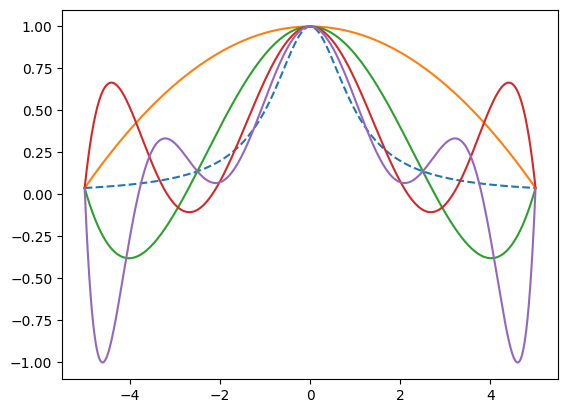
\includegraphics[width = 12cm, height = 8cm]{2.png}
	\label{fig1}
	\end{minipage}
\end{figure}

这里虚线是 $f(x)$ 的图像,黄色、绿色、红色和紫色曲线分别对应 $n=2,4,6,8$ 时的插值多项式图像。

可以看到,随着 $n$ 的增大,插值多项式没有更好地拟合 $f(x)$,反而在 $-5$ 和 $5$ 附近振荡更严重了。

\subsection{第三题,Chebyshev 插值减弱 Runge 现象}
定义函数 $f(x)=\dfrac 1{1+25x^2}$。
\begin{verbatim}
class F2 : public Function <double> {
public:
    virtual double operator () (const double &x) const {
        return 1 / (25 * x * x + 1);
    }
} f2;
\end{verbatim}

然后按题意进行求解。
\begin{verbatim}
    Newton_Interpolation<double> ip2_2 = Chebyshev_Interpolation(f2, -1, 1, 5);
    Newton_Interpolation<double> ip2_4 = Chebyshev_Interpolation(f2, -1, 1, 10);
    Newton_Interpolation<double> ip2_6 = Chebyshev_Interpolation(f2, -1, 1, 15);
    Newton_Interpolation<double> ip2_8 = Chebyshev_Interpolation(f2, -1, 1, 20);
    Polynomial<double> p2_2 = ip2_2.GetPolynomial();
    Polynomial<double> p2_4 = ip2_4.GetPolynomial();
    Polynomial<double> p2_6 = ip2_6.GetPolynomial();
    Polynomial<double> p2_8 = ip2_8.GetPolynomial();
    cout << p2_2 << endl;
    cout << p2_4 << endl;
    cout << p2_6 << endl;
    cout << p2_8 << endl;
\end{verbatim}

将输出的多项式值复制到 python 程序中,在 $[-1,1]$ 中均匀取 $1000$ 个点作图。

\begin{verbatim}
import matplotlib.pyplot as plt
import numpy as np

def f(x) :
    return 1 / (1 + 25*x**2)
def p5(x) :
    return 0.444089 -1.35642e-16*x -1.09581*x**2 +1.31782e-15*x**3 +0.711567*x**4 -1.14939e-15*x**5
def p10(x) :
    return 1 +5.55112e-16*x -12.4765*x**2 +7.10543e-15*x**3 +61.443*x**4 +1.49214e-13*x**5 -133.445*x**6 +0*x**7 +130.106*x**8 +0*x**9 -46.6329*x**10
def p15(x) :
    return 0.916893 -1.77925e-15*x -12.2846*x**2 +7.26254e-14*x**3 +83.7238*x**4 -4.11525e-14*x**5 -305.961*x**6 +2.0456e-12*x**7 +628.141*x**8 -5.30229e-12*x**9 -725.649*x**10 +2.88013e-12*x**11 +440.077*x**12 -2.57375e-12*x**13 -108.93*x**14 +6.56862e-13*x**15
def p20(x) :
    return 1 +4.94049e-15*x -21.7623*x**2 -1.06581e-14*x**3 +306.629*x**4 +1.33582e-12*x**5 -2537.27*x**6 -4.52474e-11*x**7 +12635.6*x**8 -1.47338e-10*x**9 -39333.3*x**10 +4.29281e-10*x**11 +78236.3*x**12 +1.01863e-09*x**13 -99300.1*x**14 -5.09317e-11*x**15 +77754.5*x**16 -8.73115e-11*x**17 -34208.1*x**18 -2.72848e-12*x**19 +6466.55*x**20

x = np.linspace(-1, 1, 1000)
y = [f(t) for t in x]
plt.plot(x, y, linestyle = "--")
y = [p5(t) for t in x]
plt.plot(x, y)
y = [p10(t) for t in x]
plt.plot(x, y)
y = [p15(t) for t in x]
plt.plot(x, y)
y = [p20(t) for t in x]
plt.plot(x, y)
plt.show()
\end{verbatim}

得到图像如下:

\begin{figure}[h]
    \begin{minipage}{4cm}
	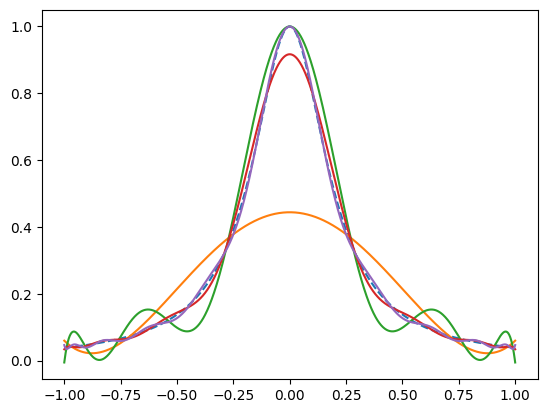
\includegraphics[width = 12cm, height = 8cm]{3.png}
	\label{fig2}
	\end{minipage}
\end{figure}

这里虚线是 $f(x)$ 的图像,黄色、绿色、红色和紫色曲线分别对应 $n=5,10,15,20$ 时的插值多项式图像。

可以发现,在 $n=20$ 时,虽然仍有微小振荡,但图像已经与 $f(x)$ 基本完全拟合。可以预见在 $n$ 更大时,图像的拟合程度应该会更高。

\subsection{第四题,车速估计}
本题已知信息为 $t=0,3,5,8,13$ 处的函数值(位移)和导数值(速度),可利用 Hermite 插值得到 $9$ 次插值多项式 $p(t)$。

\begin{verbatim}
    vector <double> x(10), y(10);
    x[0] = x[1] = 0, x[2] = x[3] = 3, x[4] = x[5] = 5, x[6] = x[7] = 8, x[8] = x[9] = 13;
    y[0] = 0, y[2] = 225, y[4] = 383, y[6] = 623, y[8] = 993;
    y[1] = 75, y[3] = 77, y[5] = 80, y[7] = 74, y[9] = 72;
    Hermite_Interpolation<double> ip3(x, y);
    Polynomial<double> p3 = ip3.GetPolynomial();
    cout << p3 << endl;
    cout << p3.d() << endl;
    cout << p3(10) << ' ' << p3.d(10) << endl;
\end{verbatim}

得到结果 $p(10)=742.503,p'(10)=48.3817$,即第一问所求 $t=10$ 时的位移和速度。

对于第二问,我们输出 $p'$ 并在 python 中对其作出图像。

\begin{verbatim}
import matplotlib.pyplot as plt
import numpy as np

def f(x) :
    return 75 +14.3238*x -30.2859*x**2 +22.0325*x**3 -7.69148*x**4 +1.45825*x**5 -0.15313*x**6 +0.00832472*x**7 -0.000182013*x**8

x = np.linspace(0, 13, 1000)
y = [f(t) for t in x]
plt.plot(x, y)
\end{verbatim}

得到图像如下(在下一页)。

\begin{figure}[h]
    \begin{minipage}{4cm}
	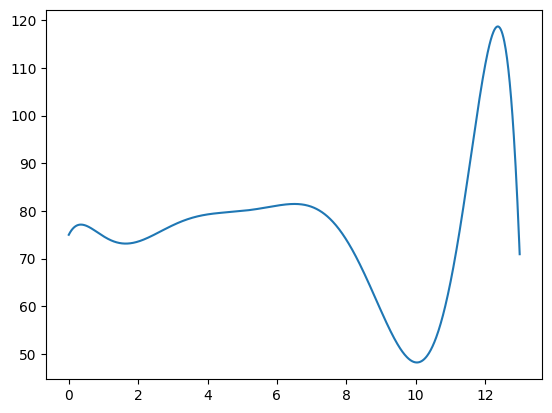
\includegraphics[width = 12cm, height = 8cm]{4.png}
	\label{fig2}
	\end{minipage}
\end{figure}

图像显示该车辆在 $t=12$ 时突然加速到 $120$ 然后又减速到 $70$,显然已经远远超过了 $81$。但个人认为本题用多项式插值去估计某点的函数值是很不准确的(也许用分段函数插值比较合理)。

\subsection{第五题,树叶生长}

本题已知信息为 $t=0,6,10,13,17,20,28$ 处的函数值。可利用 Newton 插值法得到 $6$ 次插值多项式 $p_1(t),p_2(t)$。

\begin{verbatim}
    x.resize(7);
    vector <double> y1(7), y2(7);
    x[0] = 0, x[1] = 6, x[2] = 10, x[3] = 13, x[4] = 17, x[5] = 20, x[6] = 28;
    y1[0] = 6.67, y1[1] = 17.3, y1[2] = 42.7, y1[3] = 37.3, y1[4] = 30.1, y1[5] = 29.3, y1[6] = 28.7;
    y2[0] = 6.67, y2[1] = 16.1, y2[2] = 18.9, y2[3] = 15.0, y2[4] = 10.6, y2[5] = 9.44, y2[6] = 8.89;
    Newton_Interpolation<double> ip4_1(x, y1);
    Polynomial<double> p4_1 = ip4_1.GetPolynomial();
    Newton_Interpolation<double> ip4_2(x, y2);
    Polynomial<double> p4_2 = ip4_2.GetPolynomial();
    cout << p4_1 << endl;
    cout << p4_2 << endl;
    cout << p4_1(43) << ' ' << p4_2(43) << endl;
\end{verbatim}

输出 $p_1$ 和 $p_2$ 并作图:

\begin{verbatim}
import matplotlib.pyplot as plt
import numpy as np

def p1(x) :
    return 6.67 -43.0127*x +16.2855*x**2 -2.11512*x**3 +0.128281*x**4 -0.00371557*x**5 +4.1477e-05*x**6
def p2(x) :
    return 6.67 -5.85018*x +2.98227*x**2 -0.424283*x**3 +0.0265858*x**4 -0.000777473*x**5 +8.6768e-06*x**6
x = np.linspace(0, 28, 1000)
y = [p1(t) for t in x]
plt.plot(x, y)
y = [p2(t) for t in x]
plt.plot(x, y)
\end{verbatim}

\begin{figure}[h]
    \begin{minipage}{4cm}
	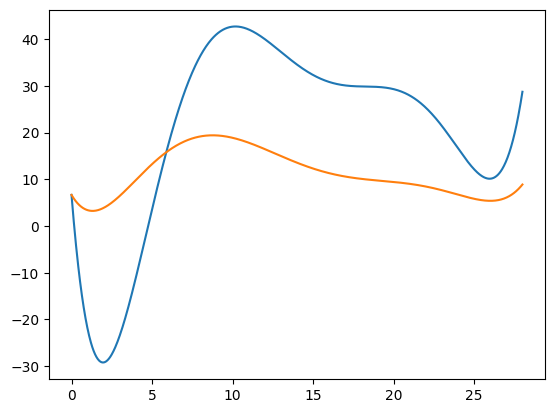
\includegraphics[width = 12cm, height = 8cm]{5.png}
	\label{fig2}
	\end{minipage}
\end{figure}

$p_2$ 的图像还比较合理,但 $p_1$ 的图像在 $t\in [1,2]$ 时竟然达到了负值!这又一次证明了多项式插值的估计是很不准确的。而多项式插值对 $t=43$ 时 $p_1,p_2$ 取值的预测更为荒谬,分别是 $p_1(43)=14640.3$ 和 $p_2=2981.48$。事实上,根据多项式的性质,在待求值点距离插值区间过远时,插值多项式的取值几乎仅与最高次项系数有关。因此用多项式插值去预测一个插值区间外的函数值是毫无意义的。

\end{document}